% !TEX encoding = UTF-8
% !TEX TS-program = pdflatex
% !TEX root = ../tesi.tex

%**************************************************************
\chapter{Descrizione dello stage}\label{cap:descrizione-stage}

\intro{In questo capitolo, viene descritto nel dettaglio il progetto di
stage, il piano di lavoro ...}

%**************************************************************

\section{Il progetto: SyncRec}

Si richiede al tirocinante, come prima parte dello stage, di apprendere le tecnologie necessari a poter svolgere le fasi di analisi, progettazione e implementazione del progetto di stage conclusivo.
Le tematiche da apprendere sono le seguenti:
\begin{itemize}
	\item \textit{Java SE} e \textit{Java EE};
	\item \textit{Database MongoDB};
	\item \textit{Spring}, nei moduli:
	\begin{itemize}[noitemsep]
		\item \textit{Spring Core};
		\item \textit{Spring Boot};
		\item \textit{Spring MVC};
		\item \textit{Spring Data MongoDB};
		\item \textit{Spring Data REST}.
	\end{itemize}
	\item Architettura a microservizi;
	\item Tecnologie per il \textit{frontend}:
	\begin{itemize}[noitemsep]
		\item \textit{Javascript};
		\item \textit{Typescript};
		\item \textit{Angular}.
	\end{itemize}
\end{itemize}

Lo studio delle tecnologie per il front-end è puramente didattico, e non è pertanto prevista una concretizzazione, compito lasciato ad altri stagisti.

La seconda parte dello stage è invece incentrata all'effettiva implementazione dei microservizi del back-end per il prodotto \textit{SyncRec} (?), il nuovo portale aziendale per la gestione delle competenze dei candidati.
 % TODO da dire di REST

Il committente di tale prodotto è l'azienda Sync Lab stessa, in quanto sarà un \textit{software} usato internamente a soli scopi burocratici.
Nello specifico, sarà lo stesso \fabio\ a coprire il ruolo di committente.

\section{Requisiti e obiettivi}

\subsection{Microservizi da sviluppare}

I microservizi accordati da implementare sono riportati nel dettaglio in seguito. Ognuno di essi esporrà le API tramite degli specifici \textit{endpoint}
raggiungibili tramite i vari tipi di richieste HTTP (GET, POST, DELETE, etc\dots).
Ogni tipo di richiesta ha la sua semantica e un significato ben specifico, che verrà spiegato nei paragrafi dedicati.
% TODO Verrà spiegato nel dettaglio nel capitolo 3 

\subsubsection{Microservizio: Email}

Il microservizio email ha il semplice compito di inviare una email specifica.
Testo, oggetto e destinatario sono dati definiti nel database MongoDB
\textit{syncrec-emailSender}, mentre le proprietà del server SMTP sono definite in un file di configurazione.

L'invio della email avviene in modo sincrono quando viene effettuata una richiesta POST tramite l'endpoint \texttt{/sendEmail}.
I parametri richiesti nel corpo della richiesta sono:
\begin{itemize}
	\item \texttt{receiver}: il destinatario della mail.
\end{itemize}

\subsubsection{Microservizio: User e Login}

Questo microservizio espone la risorsa \texttt{User} nell'endpoint
\texttt{syncrec/users}, accessibile e modificabile via API REST. I dati persistenti sono salvati e acceduti tramite il database \textit{syncrec-users} di
MongoDB.

Inoltre, tramite l'endpoint \texttt{/users/login} e una richiesta POST,
è possibile effettuare l'operazione di login.

I parametri richiesti sono:
\begin{itemize}
	\item \texttt{username}: campo contenente lo \textit{username} o l'email dell'utente che vuole autenticarsi;
	\item \texttt{password}: campo contenente la password relativa all'utente da autenticare.
\end{itemize}

Le possibili risposte che verranno inoltrate al chiamante sono:
\begin{itemize}
	\item \textbf{Ok}: 200 (Equivalente all'HTTP status \textit{ok}), e il JSON contenente i campi relativi all'utente autenticato;
	\item \textbf{Bad request}: 400 (equivalente all'HTTP status \textit{bad request}) se il corpo della richiesta non contiene i campi riportati sopra, con corpo contenente un messaggio d'errore (sempre in formato JSON);
	\item \textbf{Not found}: 404 (equivalente all'HTTP status \textit{not found}) se l'autenticazione fallisce, con corpo vuoto.
\end{itemize}

%\section{Piano di lavoro}
%Viene riportato in seguito i contenuti di maggior rilievo presenti nel piano di stage che ha pianificato
%le attività dello stesso.


\subsection{Obiettivi}

\begin{itemize}[noitemsep]
	\item Obbligatori
	\begin{itemize}
		\item \underline{\textit{O01}}: Acquisizione competenze previste dal programma;
		\item \underline{\textit{O02}}: Capacità di raggiungere gli obiettivi richiesti in autonomia seguendo il crono-programma;
		\item \underline{\textit{O03}}: Portare a termine le modifiche richieste dal cliente con una percentuale di superamento pari al 50\%.
	\end{itemize}
	\item Desiderabili
	\begin{itemize}
		\item \underline{\textit{D01}}: Portare a termine le modifiche richieste dal cliente con una percentuale di superamento pari all'80\%.
	\end{itemize}
	\item Facoltativi
	\begin{itemize}
		\item \underline{\textit{F01}}: Acquisizione competenze sul framework Spring Cloud.
	\end{itemize}
\end{itemize}

%**************************************************************

%\section{Analisi preventiva dei rischi}
%
%Durante la fase di analisi iniziale sono stati individuati alcuni possibili rischi a cui si potrà andare incontro.
%Si è quindi proceduto a elaborare delle possibili soluzioni per far fronte a tali rischi.

\begin{risk}{Performance del portatile utilizzato}
    \riskdescription{le performance del portatile, essendo ormai datato, potrebbero risultare lente o non abbastanza buone da causare dei rallentamenti sulle
        attività lavorative e di studio durante il periodo di stage}
    \risksolution{cercare di limitare gli sprechi di memoria utilizzando applicazioni non necessarie, e coinvolgere il tutor aziendale per l'eventuale sostituzione
        del PC}
    \label{risk:hardware-simulator}
\end{risk}

%**************************************************************
\section{Requisiti e obiettivi}


%**************************************************************
\section{Pianificazione}

%**************************************************************
\section{Teoria}

\subsection{Architettura software}

Da quanto si può estrapolare dallo standard IEEE 1471-2000, il concetto di architettura software può essere definito come segue:
\begin{quotation}
\noindent \textit{L'architettura software è l'organizzazione fondamentale delle componenti di un sistema, dalle relazioni che intercorrono tra esse e con l'ambiente, e i principi che ne governano la progettazione e l'evoluzione.}
\end{quotation} 

Esistono vari tipi di architettura software, ma il fine di questa sezione è quello di discutere le differenze, i pro e i contro tra un'architettura tradizionale monolitica e la ben più recente architettura a microservizi.

\subsubsection{Architettura monolitica}

\begin{figure}[H]
	\centering
%	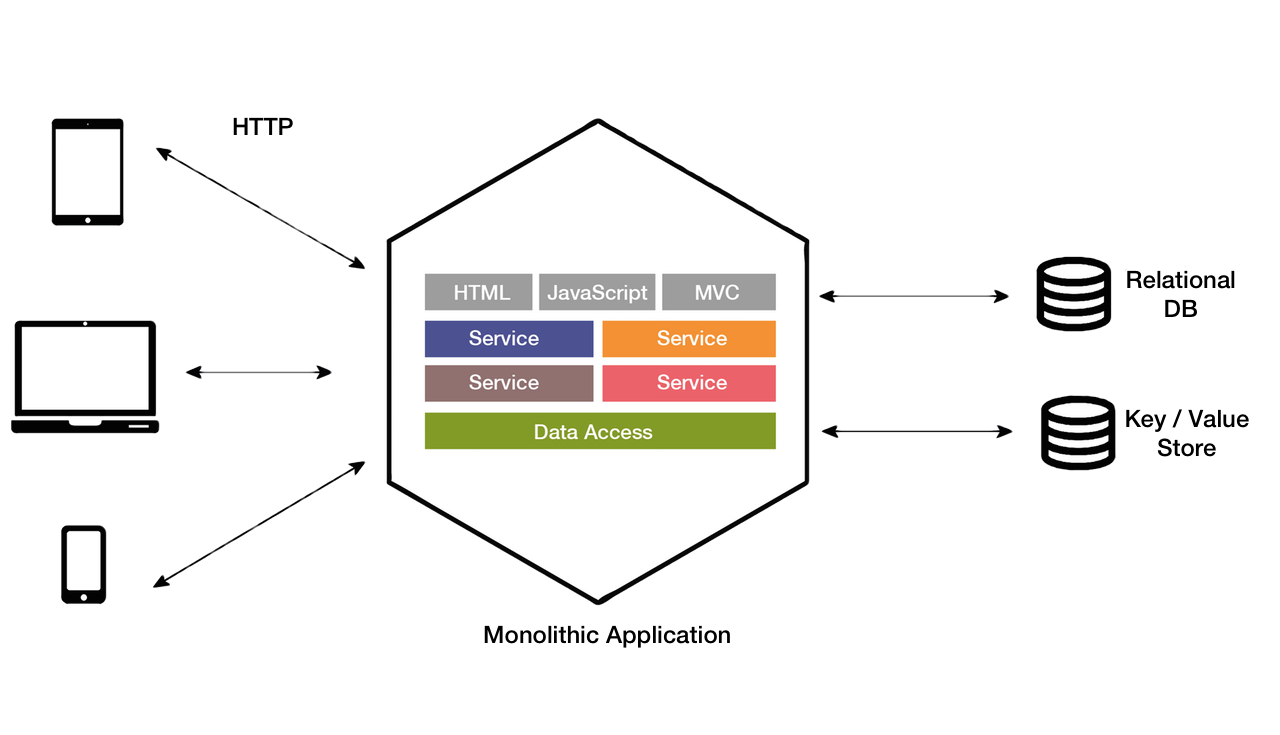
\includegraphics[width=\textwidth/2]{immagini/monolithic_architecture.png} % FONTE: https://medium.com
	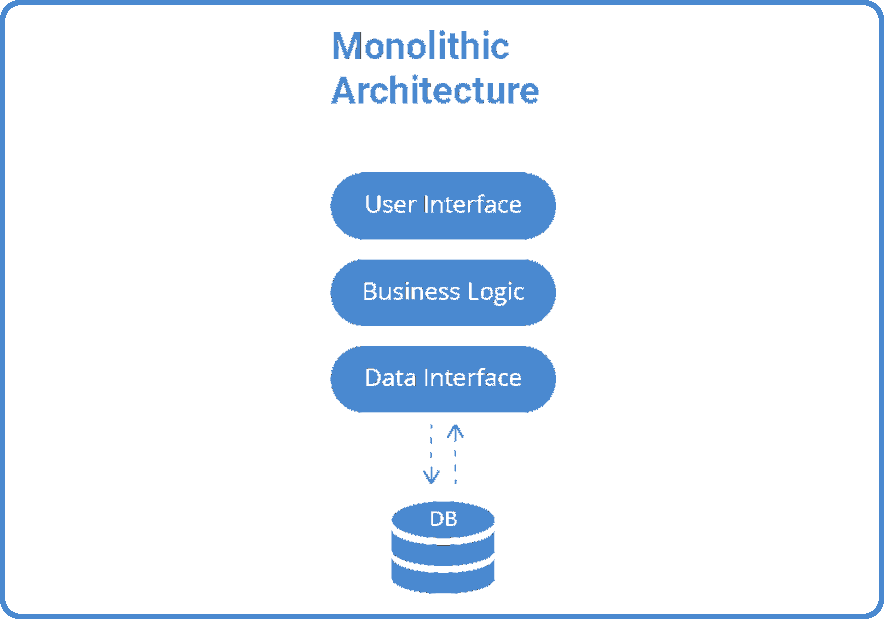
\includegraphics[width=0.4\textwidth]{immagini/monolithic_architectureB.png} % FONTE: https://www.sam-solutions.com/blog/microservices-vs-monolithic-real-business-examples/
	\caption[Architettura monolitica]{Architettura monolitica\footnotemark}
\end{figure}
\footnotetext{Fonte immagine: \href{https://www.sam-solutions.com/blog/microservices-vs-monolithic-real-business-examples/}{https://www.sam-solutions.com}}
